%Template pembuatan proposal skripsi.
\documentclass{jtetiproposalskripsi}

%-----------------------------------------------------------------
%Disini awal masukan untuk data proposal skripsi
%-----------------------------------------------------------------
\titleind{PERANCANGAN SISTEM DETEKSI GAS LPG MELALUI WEB BERBASIS OPENWRT}

\fullname{GUFRON ALFIAN RIFA'I}

\idnum{111065 1159}

\approvaldate{20 Desember 2014}

\degree{Sarjana Teknik Informatika}

\yearsubmit{2014}

\program{Teknik Informatika}

\headprogram{Sarjiya, S.T., M.T., Ph.D.}

\dept{Teknik Informatika}

\firstsupervisor{Sigit Basuki Wibowo, S.T., M.Eng.}
\firstnip{1976 0501 2002 12 1 002}

\secondsupervisor{Bimo Sunarfri Hantono, S.T., M.Eng.}
\secondnip{1977 0131 2002 12 1 003}


%-----------------------------------------------------------------
%Disini akhir masukan untuk data proposal skripsi
%-----------------------------------------------------------------

\begin{document}

\cover

\approvalpage

%-----------------------------------------------------------------
%Disini akhir masukan untuk muka skripsi
%-----------------------------------------------------------------

%-----------------------------------------------------------------
%Disini awal masukan Intisari
%-----------------------------------------------------------------
\begin{abstractind}
Kelangkaan minyak tanah membuat masyarakat gelisah. Karena minyak tanah metupakan kebutuhan pokok untuk memasak sehari-hari. Maka dari itu masyarakat Indonesia berbondong-bondong beralih dari minyak tanah menggunakan gas LPG. Kafrena gas LPG lebih murah dibandingkan dengan minyak tanah. Dibalik penggunaan LPG dari segi harga yang murah dan penggunaannya yang efisien dari minyak tanah , korban gas LPG sering disebabkan oleh kebocoran pipa dan instalasi regulator yang tidak tepat. Oleh karena itu, perlu untuk membangun sebuah sistem yang memiliki fitur dapat mendeteksi gas LPG untuk memberikan kenyamanan bagi penggunanya.

Sistem ini dibangun dengan memanfaatkan sistem operasi OpenWRT. Sistem operasi OpenWRT akan dipasang pada router nirkabel dengan beberapa alat tambahan untuk mendukung fungsi seperti sensor deteksi gas, Arduino, modem gsm, speaker, flash, dll.

Sistem yang dihasilkan akan memiliki kemampuan untuk mendeteksi gas LPG, sistem ini juga mampu memberikan peringatan dalam bentuk alarm peringatan, peringatan melalui SMS, dan kemudahan akses melalui LAN dan WIFI


\bigskip
\textbf{Kata kunci} : OpenWRT, Router Wireless, Arduino.
\end{abstractind}
%-----------------------------------------------------------------
%Disini akhir masukan Intisari
%-----------------------------------------------------------------

\tableofcontents
\addcontentsline{toc}{chapter}{DAFTAR ISI}
\selectlanguage{bahasa}\clearpage\pagenumbering{arabic}\setcounter{page}{1}

%-----------------------------------------------------------------
%Disini awal masukan untuk Bab
%-----------------------------------------------------------------
\chapter{LATAR BELAKANG}

\section{Latar Belakang Masalah}
Dalam bahasa yang paling sederhana, home automation atau otomatisasi rumah dapat digaumber daya alam yang bermanfaat bagi kehidupan manusia sangatlah banyak tersedia di bumi ini. Baik itu sumber daya alam yang dapat diperbaharui maupun sumber daya alam yang tidak diperbaharui. gas LPG (Liquefied Petroleum Gas) merupakan salah satu hasil dari sumber daya alam yang tidak dapat diperbaharui. Peranan gas LPG pada saat ini sangatlah penting bagi kehidupan manusia. Teringat, semakin menipisnya persediaan minyak dibumi ini perlahan–lahan gas LPG mulai menggantikan peranan utama dari minyak bumi sebagai bahan bakar altetnatif baik itu dalam bidang industri, rumah tangga, maupun transportasi.

Terkadangkala manusia terbuai akan kayanya sumber daya alam ini. Disaat sengaja maupun tidak sengaja, gas LPG dapat menjadi dampak negatif terhadap kesehatan manusia bahkan menimbulkan kerugian yang cukup besar apabila tidak digunakan dengan hati – hati terutama bila tidak diketahui telah terjadinya kebocoran dari tabung atau tempat penyimpanan gas LPG. Seharusnya, gas LPG tersebut sesuatu yang dapat mempermudah kelangsungan hidup manusia tetapi menjadi kerugian manusia. Pada saat ini banyak terjadi insiden ledakan gas LPG yang di akibatkan oleh kebocoran gas lpg dan yang paling parah kebakaran serta ledakan. 

Seiring dengan perkembangan ilmu dan teknologi maka dikembangkan sebuah sistem keamanan dengan cara memberikan peringatan (warning system). untuk memberikan sebuah tanda jika ada tercium bau gas disekitar rumah. Jika sistem ini mendeteksi adanya bau gas LPG maka sistem ini akan memberikan sebuah tanda berupa alarm dan sebuah pesan singkat atau Short Message Service (SMS) yang akan dikirim ke nomor telepon seluler (handphone) sehingga dapat mengetahui adanya gas bocor di rumah.
 



\section{Tujuan Penelitian}
Adapun tujuan dari penelitian ini adalah Membuat system memiliki kemampuan untuk mendeteksi gas LPG, sistem ini juga mampu memberikan peringatan dalam bentuk alarm peringatan, peringatan melalui SMS, dan kemudahan akses melalui LAN dan WIFI.


\section{Manfaat Penelitian}
Manfaat dari penelitian ini adalah mempermudah pengguna dalam melakukan pengawasan terhadap gas LPG sehingga tindakan pencegahan terhadap hal-hal yang tidak diinginkan dapat dilakukan secepatnya.
 

%-------------------------------------------------------------------------------
\chapter{TINJAUAN PUSTAKA DAN DASAR TEORI}                

\section{Tinjauan Pustaka}
Openwrt digunakan sebagai sistem operasi yang berjalan pada router. Openwrt merupakan sistem operasi berbasis Linux yang bersifat open-source, sehingga dapat di konfigurasi agar berjalan sesuai dengan kebutuhan pada penelitian ini. Aplikasi untuk kendali sistem otomatisasi perangkat listrik rumah akan berjalan pada web server yang terdapat didalam Openwrt yang dapat mengenali perangkat mikrokontroller Arduino yang terhubung melalui USB.

Oleh karena itu dalam penelitian ini digunakan sistem operasi Linux untuk embedded device yang bernama Openwrt, sebuah router, sebuah rangkaian mikrokontroller Arduino, rangkaian relay dan beberapa sensor untuk membangun sebuah sistem yang dapat digunakan untuk otomatisasi rumah dengan biaya yang relatif murah, hemat daya listrik dan dapat diakses dari jarak jauh karena memiliki antarmuka pengguna berbasis web yang dapat diakses menggunakan berbagai macam perangkat, baik melalui jaringan internet ataupun jaringan lokal.


\section{Landasan Teori}
\subsection{Definisi Arduino Uno }
Arduino Uno adalah salah satu produk berlabel arduino yang sebenarnya adalah suatu papan elektronik yang mengandung mikrokontroler ATmega328 (sebuah keeping yang secara fungsional bertindak seperti sebuah komputer). Piranti ini dapat dimanfaatkan untuk mewujudkan rangkaian elektronik dari yang sederhana hingga yang kompleks.



\subsection{Daya Eksternal}
Arduino Uno dapat disuplai melalui koneksi USB atau dengan sebuah power suplai eksternal. Sumber daya dipilih secara otomatis. Suplai eksternal (non-USB) dapat diperoleh dari sebuah adaptor AC ke DC atau battery. Adaptor dapat dihubungkan dengan mencolokkan sebuah center-positive plug yang panjangnya 2,1 mm ke power jack dari board.

\subsection{Karakteristik Fisik}
Panjang lebar maksimum dari PCB Arduino Uno masing-masing adalah 2.7 dan 2.1 inci, dengan konektor USB dan power jack yang memperluas dimensinya. Empat lubang sekrup memungkinkan board untuk dipasang ke sebuah permukaan atau kotak. Jarak antara pin 7 dan 8 adalah 160 mili (0.16 inch).



\subsection{Arduino IDE}
Arduino IDE adalah lingkungan pengembangan arduino yang berisi teks editor untuk menuliskan kode, pesan area, teks console, toolbar dengan tombol fungsi umum, dan serangkaian menu. Terhubung ke perangkat keras yang terhubung ke perangkat arduino board dan berkomunikasi dengan board tersebut. Perangkat lunak yang dituliskan menggunakan arduino disebut sketch, sketch ini ditulis dalam editor teks. Teks editor memiliki fitur copy/paste dan mencari/mengganti teks. Area pesan memberikan umpan balik saat menyimpan dan mengekspor dan juga menampilkan kesalahan yang terdapat dalam kode program.

\subsection{Jaringan Komputer}
Jaringan komputer (Computer Network) yang disebut secara singkat dengan jaringan adalah kumpulan komputer dan alat-alat lain yang saling dihubungkan bersama menggunakan media komunikasi tertentu.
Komputer dalam jaringan dapat saling berhubungan melalui kabel,jaringan telepon,gelombang radio, satelit ataupun sinar infra merah. Ada tiga tipe jaringan dalam hubungannya dengan luas area yang dicakup yaitu:
 
1. LAN (Local Network Area)

2. MAN (Metropolitan Area Network)

3. WAN (Wide Area Network)

\subsection{Jaringan WLAN}
Jaringan WLAN (Wireless LAN) adalah jaringan LAN yang tidak menggunakan kabel sebagai media transmisi data. (Wagito 2007:14) Jaringan ini menggunakan gelombang elektromagnetik dalam melakukan transfer data. Jaringan WLAN di dasarkan pada standar IEEE 802.11. Perkembangan awal jaringan WLAN hanya mampu melakukan transfer data maksimum sampai 2 Mbps.

\subsection{HTML (HyperText Mark up Language)}
HTML adalah bahasa pemrograman yang digunakan untuk membuat sebuah halaman web, yang kemudian dapat diakses untuk menampilkan berbagai informasi di dalam sebuah web internet (Browser) . HTML dapat juga digunakan sebagai link antara file-file dalam situs atau dalam komputer dengan menggunakan localhost.

\subsection{Pemrograman PHP}
PHP (hypertext Preprocessor) adalah bahasa skrip yang ditanamkan atau disisipkan ke dalam HTML. PHP banyak dipakai untuk memprogram situs web dinamis. PHP dapat digunakan untuk membangun sebuah CMS.3 Salah satu keunggulan PHP dibanding dengan bahasa pemograman yang lain adalah PHP merupakan bahasa pemograman opensource dan dapat diperoleh secara gratis. Walaupun gratis, namun PHP sangat powerfull. Dibuktikan dengan banyaknya website yang menggunakan PHP. PHP juga sudah mendukung OOP (Object Oriented Programming) sehingga maintenance kode menjadi lebih mudah.

\subsection{MySQL}
MySQL adalah sebuah perangkat lunak sistem manajemen basis data SQL (database management system) atau DBMS yang multithread, multiuser, dengan sekitar 6 juta instalasi di seluruh dunia. MySQL AB membuaat MySQL tersedia sebagai perangkat lunak gratis dibawah lisensi GNU General Public License(GPL), tetapi mereka juga menjual dibawah lisensi komersial untuk kasus-kasus dimana penggunaanya tidak cocok dengan penggunaan GPL.

\subsection{SSH (Scure Shell)}
SSH (Secure Shell) adalah Program ssh di gunakan untuk login dalam suatu mesin (komputer) dari jauh (secara remote) dan mengeksekusi perintah pada mesin tersebut. (Wagito 2007:239) Program ssh ini mirip dengan telnet, tetapi punya pengendalian terhadap keamanan. Program ssh menyediakan komunikasi aman terenkrip antara dua host yang berada dalam jaringan sehingga memiliki keamanan yang lebih terjamin daripada telnet.

\subsection{SMS Gateway}
Istilah gateway, bila dilihat pada kamus Inggris-Indonesia diartikan sebagai pintu gerbang. Namun pada dunia komputer, gateway dapat berarti juga sebagai jembatan penghubung antar satu sistem dengan sistem lain yang berbeda, sehingga dapat terjadi suatu pertukaran data antar sistem tersebut. Dengan demikian, SMS gateway dapat diartikan sebagai suatu penghubung untuk lalu lintas data-data SMS, baik yang dikirimkan maupun yang diterima. Sebuah gateway SMS adalah cara mengirim pesan teks dengan atau tanpa menggunakan telepon seluler.

\subsection{Firmware}
Firmware (Perangkat Tegar) merupakan perangkat lunak yang sengaja ditanamkan secara semi permanen. contoh dari firmware terdapat pada BIOS, CISCO access point, router, handphone. Firmware bisa disebut sebagai sistem operasi yang ditanam Embedded Operating System dan biasanya disimpan dalam flash ROM dari perangkat keras.

\subsection{Flowchart}
Flowchart adalah penyajian yang sistematis tentang proses dan logika dari kegiatan penanganan informasi atau pengGambaran secara grafik dari langkah-langkah dan urut-urutan prosedur dari suatu program. Flowchart menolong analis dan programmer untuk memecahkan masalah kedalam segmen-segmen yang lebih kecil dan menolong dalam menganalisis alternatif-alternatif lain dalam pengoperasian. System flowchart adalah urutan proses dalam system dengan menunjukkan alat media input, output serta jenis media penyimpanan dalam proses pengolahan data. Program flowchart adalah suatu bagan dengan simbol-simbol tertentu yang mengGambarkan urutan proses secara mendetail dan hubungan antara suatu proses (instruksi) dengan proses lainnya dalam suatu program.


%-------------------------------------------------------------------------------
\chapter{METODOLOGI}

\section{Alat dan Bahan}
Pada perancangan ini merupakan bagian yang sangat rentan terhadap kerusakan dan kesalahan dalam pembuatan. Oleh karena itu diperlukan ketelitian dalam pengerjaan sistem ini. Sebelum kearah pembuatan rancangan deteksi gas LPG melalui web, maka diperlukan alat-alat yang mendukung sistem ini.

\begin{figure}[ht!]
  \centering
    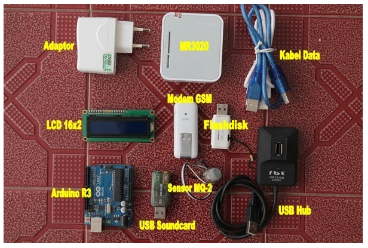
\includegraphics{gambar/1}
    \caption{Alat-alat yang dibutuhkan}
    \label{1}
\end{figure}

\section{Langkah Kerja}

Untuk mendapatkan data dan informasi yang baik dan tepat, maka penulis menggunakan teknik sebagai berikut:

\textbf{1. Analisis Sistem}

Analisis sistem dapat didefinisikan sebagai penguraian dari suatu sistem informasi yang utuh kedalam bagian-bagian komponennya dengan maksud untuk mengidentifikasi kesempatan, dan mengevaluasi hambatan-hambatan, kesempatan-kesempatan permasalahan-permasalahan, yang terjadi dan kebutuhan-kebutuhan yang diharapkan sehingga dapat diusulkan perbaikan-perbaikannya. kesempatan-

\textbf{2. Perancangan}

Sistem deteksi gas LPG yang akan dibangun memiliki fitur khusus yaitu dapat dikendalikan melalui perangkat wireless yang memiliki aplikasi web yang bisa mengakses perangkat ini. Karena semua perangkat wireless yang terhubung telah dikoneksikan pada sistem ini, maka akan didapat hasil dari tujuan yang diinginkan. Maka dari itu dibutuhkan suatu bentuk pengaman yang bisa dilakukan supaya kebakaran rumah bisa diminimalisir serta mendapat informasi dini terjadi kebocoran gas oleh pemilik rumah.

Salah satu bentuk pengaman adalah dengan menggunakan suatu metode, teknik, cara, atau teknologi yang berbasis OpenWRT. Sehingga rumah yang telah terpasang sistem ini tetap merasa aman dan terkendali dari hal-hal yang tidak kita inginkan ketika meninggalkan rumah untuk bekerja dan berbelanja.
Tahapan ini dilakukan persiapan softeware yang mendukung dalam perancangan sistem jaringan.

\textbf{3. Implementasi}

Pada tahap ini, hasil perancangan sistem maupun perancangan antarmuka akan diimplementasikan dengan menggunakan PHP dan bash script.

\textbf{4. Pengujian}

Pada pengujian sistem deteksi gas LPG pada penelitian ini menggunakan sensor gas MQ-2 dengan korek gas. Pada dasarnya gas yang ada didalam korek gas juga berasal dari isi tabung gas. Karena kandungan isi korek gas tidak jauh beda dengan isi tabung LPG tersebut.

\begin{figure}[ht!]
  \centering
    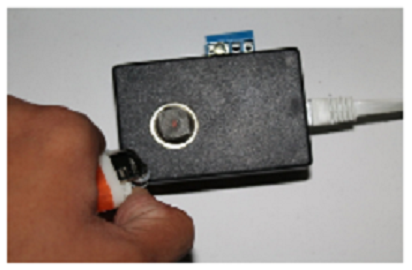
\includegraphics{gambar/2}
    \caption{Uji coba dengan korek gas}
    \label{1}
\end{figure}


\section{Jadwal Kegiatan}
Penelitian direncanakan akan dilaksanakan selama enam bulan. Rincian rencana jadwal penelitian dicantumkan dalam tabel berikut.

\begin{center}
Tabel Jadwal Penelitian.
\end{center}
\vspace{-0.5cm}
\begin{figure}[ht!]
  \centering
    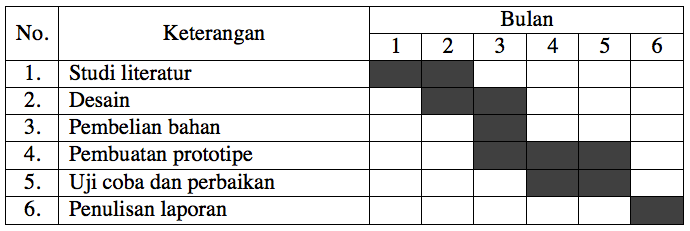
\includegraphics[width=13cm]{gambar/timeline}
\end{figure}

%-----------------------------------------------------------------
%Disini akhir masukan Bab
%-----------------------------------------------------------------

%-----------------------------------------------------------------
%Disini awal masukan untuk Daftar Pustaka
%-----------------------------------------------------------------
%%\nocite{Abel2010,Guerbas201350}
%%\bibliography{research-plan}
%%\bibliographystyle{plainnat}
\begin{thebibliography}{9}

\bibitem[satu(2014)]{satu01}

Al Fatah, Hanif. 2007. Analisis dan Perancangan Sistem Informasi untuk Keunggulan Bersaing Perusahaan dan Organisasi Modern. Yogyakarta : Penerbit Andi

\bibitem[dua(2014)]{dua02}
Arduino Uno Board. http://arduino.cc/en/Main/arduinoBoardUno. (diakses tanggal 4 Maret 2014)

\bibitem[tiga(2014)]{tiga03}
Bash Shell. http://themoxstar-tms.blogspot.com/2013/03/pengertian-bash.html, (diakses tanggal 8 Maret 2014)


\end{thebibliography}
\addcontentsline{toc}{chapter}{DAFTAR PUSTAKA}
%-----------------------------------------------------------------
%Disini akhir masukan Daftar Pustaka
%-----------------------------------------------------------------

\end{document}